\documentclass[10pt,twocolumn]{article}
\usepackage[margin=0.75in]{geometry}
\usepackage{amsmath,amssymb,amsthm,booktabs,graphicx,hyperref,microtype,xcolor}
\newcommand{\system}{ContourMark}
\newtheorem{proposition}{Proposition}
\newtheorem{theorem}{Theorem}
\title{\system: Blind, Representation-Invariant Watermarking of SVG Geometry}
\author{Anonymous submission draft}
\date{30 September 2026}

\begin{document}
\maketitle

\begin{abstract}
Language models and specialist generators now emit SVG code at scale, and regulation (EU AI Act Art.~50) asks providers to mark AI-generated content in a machine-readable way. Current practice for SVG is signed metadata, which the default configuration of the dominant optimizer (SVGO) deletes. Token-level LLM watermarks fail for the same reason: SVG toolchains rewrite nearly every token while preserving the picture. We present \system{}, a blind watermark carried by the drawn geometry itself. Each contour is resampled by arc length. The magnitudes of a band of Fourier (or cosine) coefficients of its normalized radial function are invariant to command syntax, segment subdivision, path merging and reordering, start point, direction, and similarity transforms. A keyed dither-modulation quantizer moves these magnitudes onto a secret lattice. A representation-free capacity model lets the detector decide, from the observed geometry alone, which coefficients a contour could have carried. Detection needs only the SVG and the key. It reports a p-value that is a valid upper bound over the key's randomness for any SVG chosen independently of the key, computed exactly by an exponentially tilted convolution rather than fitted to data. On 900 icons, logos, and emoji from nine open-license sets, 83\% of marked assets are detected at $p\le10^{-6}$ from the SVG and key alone. The misses are mostly icons with at most one curved contour. Of the detectable assets, 94\% survive default SVGO, 100\% survive Scour, and 100\% survive rotation, scaling, mirroring, reordering, subdivision, and path merging or splitting. Metadata, XML-comment, coordinate-LSB, Bézier-split, and vertex Fourier-descriptor baselines all fail under SVGO, rounding, or similarity transforms. Over 268{,}200 key-randomized null tests the empirical false-positive rate tracks the bound from $10^{-1}$ to $10^{-5}$. On SVGs written by a local LLM, detection is 100\% clean and 100\% after SVGO. We report the failure boundary as prominently as the successes: noise at the mark's amplitude, aspect-ratio stretching, stroke outlining, rasterize-and-retrace, an informed re-quantization attacker, and icons made only of straight lines.
\end{abstract}

\section{Introduction}
SVG is both a program and a picture. The same rendering admits absolute or relative commands, shorthand curves, arbitrary numeric precision, merged or split paths, group transforms, and basic shapes instead of paths. Production pipelines exercise all of this freedom. SVGO, the default optimizer in web build chains, rounds coordinates, rewrites commands, merges paths, and strips metadata and comments. As a result, a provenance signal stored in syntax (a C2PA manifest, an XML comment, least-significant digits, a segment-split pattern) disappears on the first build.

The problem is becoming practical. Code-writing LLMs routinely produce SVG. Specialist models (StarVector, OmniSVG, InternSVG) generate icons and illustrations. Article~50 of the EU AI Act, applicable from August 2026, requires machine-readable marking of AI-generated content. Text watermarks that bias token sampling do not transfer: an SVG optimizer is a near-total semantics-preserving rewrite of the token stream, the extreme case of the code-rewriting attacks that already defeat code watermarks.

\system{} moves the mark from tokens to \emph{drawn geometry}. It is applied post hoc, so it covers every generator with the same code and needs no model access. Our contributions are:
\begin{enumerate}
\item \textbf{A representation-invariant carrier.} The band magnitudes of a contour's arc-length radial function do not depend on how the contour is encoded (\S\ref{sec:carrier}).
\item \textbf{Keyed QIM with content-seeded dithers and a representation-free capacity model.} The verifier recomputes, from geometry alone, which coefficients a contour can carry. A structure-preserving embedder realizes the mark on the file's own control points (\S\ref{sec:embed}).
\item \textbf{An exactly calibrated blind detector.} It returns a valid p-value bound over key randomness, computed by tilted discretized convolution, and combines a dense test with a Bonferroni per-contour test for composed documents (\S\ref{sec:detect}).
\item \textbf{A corpus-scale evaluation} on 900 real assets and LLM-generated SVG. It covers 36 keyless transformations, four re-implemented prior schemes, fidelity and size costs, a million-test null calibration, and an informed attacker (\S\ref{sec:eval}).
\end{enumerate}
A zero-distortion generation-time variant for generators that expose candidate choices is described in \S\ref{sec:gen}.

\section{Threat model and goals}
\label{sec:threat}
A provider holds a secret key $K$. It marks SVGs before release, and later tests a suspect file with $K$ alone (no original, database, or manifest). We distinguish three adversaries:
\begin{itemize}
\item \textbf{A0 (benign processing):} optimizers (SVGO, Scour, picosvg), precision reduction, format normalization, similarity transforms, reordering, merging and splitting, subdivision, composition into larger artwork, cropping.
\item \textbf{A1 (keyless editing):} coordinate noise, simplification to polylines, non-uniform scaling, rasterize-and-retrace.
\item \textbf{A2 (informed, keyless):} knows the algorithm and public parameters but not $K$; for example, re-embeds with a random key.
\end{itemize}
We claim robustness only for named transformations and report A1/A2 failure boundaries. Following the impossibility results of Zhang et al., we make no claim against attackers with a quality oracle and unbounded edits.

\textbf{False attribution} is the primary security requirement. The probability that an SVG chosen independently of $K$ is declared marked must be at most the stated $\alpha$, without assumptions about the SVG distribution. Keys and asset identifiers should be committed before release if detection is used as evidence. Invisible geometry is excluded from detection so that hidden marked decoys cannot authenticate unrelated visible content.

\section{Design}
\subsection{Carrier: radial-function spectra}
\label{sec:carrier}
For each visible contour $c$ (after flattening transforms and converting shapes), we sample $N=256$ points $p_n$ uniformly by arc length. We then form the normalized radial function
\[
\rho_n=\frac{|p_n-\bar p|}{\frac1N\sum_m|p_m-\bar p|},\qquad \bar p=\tfrac1N\textstyle\sum_n p_n .
\]
For closed contours the carrier is $m_k=2|\hat\rho_k|$, where $\hat\rho$ is the DFT, for $k=2,\dots,9$. For open contours it is the magnitude of DCT-II coefficients.

\begin{proposition}
The carrier is invariant, up to resampling error, to: path command syntax and precision-preserving rewrites; exact subdivision of segments; path merging, splitting and reordering; the start point and direction of closed contours; the direction of open contours; translation, uniform scaling, rotation and reflection.
\end{proposition}
\emph{Proof sketch.} Arc-length samples depend only on the drawn curve. Translation and scale are removed by centering and normalization, and rotation and reflection leave $|p-\bar p|$ unchanged. A change of start point is a cyclic shift and a reversal is an index reversal; DFT magnitudes are invariant to both, and DCT-II magnitudes are invariant to reversal. \qed

Curves are sampled with a per-segment budget proportional to length, so the chord error is nearly independent of how the curve is split. Without this, arc-versus-cubic encodings differed by $10^{-3}$ in $\rho$, a quarter of the lattice step.

\subsection{Keyed lattice and content-seeded dithers}
\label{sec:embed}
Each contour receives a seed $s(c)$: a coarse, similarity-invariant shape class (quantized log isoperimetric or straightness ratio and log elongation). The dithers are $d_{s,k}=\mathrm{PRF}_K(s,k)\in[0,1)$. The embedder moves each carried magnitude to the nearest point of $\Delta(\mathbb Z+d_{s,k})$, with $\Delta=0.004$ (in units of the mean radius). Seeding by content means an attacker cannot pool unrelated contours to estimate one lattice. Seed collisions within a document are handled exactly by the detector (\S\ref{sec:detect}).

\textbf{Capacity from geometry.} A circle drawn with four cubics cannot carry high-frequency ripple on its handles, and a polygon's straight edges must stay straight. We define a \emph{geometric deformation model} on the samples. Curved stretches move along their normals under a low-frequency field; exactly straight runs interpolate their endpoint motion, so lines stay lines. Coefficient $k$ is carried if its magnitude Jacobian row, orthogonalized against lower frequencies, has norm $\ge 0.4$. The rule depends only on geometry, so the verifier recomputes it after any rewrite. The embedder marks the superset with gain $\ge0.25$ (hysteresis).

\textbf{Structure-preserving realization.} The embedder moves the file's own handles by a low-frequency normal field. It solves for the field with minimum-norm Gauss--Newton on the complex coefficients. Where a magnitude is zero it linearizes along the direction of largest gain; every band coefficient of a circle is such a case. Curved segments are split, exactly, only when the handles cannot realize a selected coefficient. Arcs are converted to $\le 45^\circ$ cubics, because moving an arc's endpoints keeps it rigid. Output precision is chosen per element so that rounding stays below $0.05\,\Delta\bar r$. Lines stay lines, other elements and attributes are untouched, and comments are preserved.

\subsection{Detection and exact calibration}
\label{sec:detect}
Contours sharing a seed share dithers, so they are pooled. For group $g$ and coefficient $k$, let
\[
A_{g,k}=\sum_{c\in g}\mathbb 1[k\text{ selected for }c]\,e^{2\pi i m_{c,k}/\Delta},
\qquad
T=\sum_{g,k}\operatorname{Re}\big(A_{g,k}e^{-2\pi i d_{g,k}}\big).
\]
\begin{theorem}
Let an SVG be fixed independently of $K$, and model the PRF as random. Then $T\stackrel{d}{=}\sum_{g,k}|A_{g,k}|\cos(2\pi U_{g,k})$ with $U_{g,k}$ i.i.d.\ uniform. Hence any upper bound $\bar P(t)\ge\Pr[\sum w_i\cos 2\pi U_i\ge t]$ with $w=|A|$ yields a p-value satisfying $\Pr[\bar P(T)\le\alpha]\le\alpha$.
\end{theorem}
\emph{Proof.} Given the document, the $A_{g,k}$ are fixed. Distinct $(g,k)$ have independent uniform dithers, and a uniform phase shift of a fixed phasor gives a uniform angle. \qed

We compute $\bar P$ exactly rather than asymptotically. Each term $w\cos(2\pi U)$ is rounded \emph{up} to a grid. The discretized sum then stochastically dominates $T$, so its tail is a valid bound. We exponentially tilt each term by the Chernoff-optimal $\theta$, convolve by FFT (so floating point is accurate near $t$), and untilt. The reported bound is the minimum of this value and the Chernoff bound. Against $2\times10^6$ Monte Carlo draws it is within 10\% of the truth and never below it; Chernoff alone is about $5\times$ conservative.

\textbf{Composition.} A marked icon pasted among unmarked artwork dilutes $T$. We therefore also compute a per-contour bound $p_c$ and use $p=2\min(\bar P(T),\,C\min_c p_c)$, which is valid by the union bound under any dependence. This raised the detection of a composed stroke icon from $10^{-2}$ to $10^{-10}$.

\section{Zero-distortion generation-time variant}
\label{sec:gen}
When a generator proposes $m$ candidate contours with probabilities $q_i$, a keyed Gumbel-max draw $J=\arg\max_i \log q_i-\log(-\log u_i)$ with $u_i=\mathrm{PRF}_K(\cdot)$ preserves the output distribution and moves no geometry. Verification needs a private authenticated candidate manifest; the repository's \texttt{sample}/\texttt{verify-sample} implement it with a Poisson-binomial test. In three 16-step Qwen-generated drawings all keyed choices verified after SVGO, Scour, rounding, reordering, and bounded translation. This variant suits generators that expose candidate choices or coordinate logits, such as the tokenized coordinates of OmniSVG. The blind scheme above suits every generator.

\section{Evaluation}
\label{sec:eval}
\subsection{Setup}
\textbf{Corpus.} 900 test assets, 100 from each of nine open-license sets: Lucide and Tabler (stroked line icons); Bootstrap, Material, Font Awesome, Remix, and Octicons (filled icons); Simple Icons (logos); and OpenMoji (colour illustrations). A disjoint 270-asset development split, separated by filename hash, was used for all tuning. Parameters were frozen before any test-split run. We also use 40 SVGs written by a local LLM (Qwen~3.5 4B through Ollama) from icon prompts.

\textbf{Methods.} We compare \system{} (defaults $\Delta{=}0.004$, $k{=}2..9$) with: an XML comment; a \texttt{<metadata>} credential standing in for C2PA; geometry-aware coordinate-parity LSB (64 chips at $10^{-3}$); Bézier-split steganography; and a vertex Fourier-descriptor magnitude watermark with correlation detection (Solachidis/Doncel/Pitas). The detection threshold for all methods is $p\le10^{-6}$.

\textbf{Attacks (36, all keyless):}
\begin{itemize}
\item optimizers: SVGO (default, multipass, precision 2 and 1), Scour (default, precision 3), picosvg;
\item absolute rounding to 2, 1, and 0 decimals;
\item similarity: translate, scale $\times0.37$ and $\times3$, rotate $30^\circ$ and $90^\circ$, mirror, nested group transform;
\item non-uniform $1.2{:}1$ stretch;
\item structure: reorder, reverse, restart, exact subdivision, merge, split;
\item deletion of 25\% or 50\% of contours, half crop, composition into a $2{\times}2$ grid with unmarked icons;
\item Gaussian handle noise at 0.1, 0.3, and 1\% of the diagonal;
\item flattening to polylines with Douglas--Peucker simplification;
\item rasterize (librsvg, 512 or 1024\,px) and retrace (potrace).
\end{itemize}

\subsection{Detection and robustness}
\system{} detects 83\% of marked test assets (747/900) with no attack. Across sources this ranges from 69\% (Lucide) and 70\% (Tabler), which are mostly straight strokes, to 92\% (OpenMoji). Among the 153 misses:
\begin{itemize}
\item 56 have at most one markable contour;
\item the median miss still reaches $p=1.6\times10^{-4}$;
\item 92 reach $p\le10^{-3}$.
\end{itemize}
Capacity, not robustness, limits coverage. The embedder reports the attainable $p$ in advance, so a provider knows when an asset cannot be marked.

Conditional on clean detection, survival rates with 95\% Wilson intervals are:
\begin{itemize}
\item SVGO default 94.2\% [92.3, 95.7]; SVGO multipass 94.4\%;
\item Scour 100\% [99.5, 100]; picosvg 78.3\%;
\item 2-decimal rounding 77.2\%;
\item all seven similarity transforms 100\%;
\item reorder, reverse, subdivide, merge, split 100\%; restart 95.9\%;
\item deleting 25\% of contours 97.1\%; half crop 82.3\%; composition 89.2\%;
\item light polyline flattening (0.05\% tolerance) 83.1\%.
\end{itemize}
Figure~\ref{fig:attacks} compares attack families.

The failure boundary is equally clear:
\begin{itemize}
\item 1-decimal rounding: 14.6\%;
\item SVGO precision 1: 8.8\%;
\item handle noise at 0.1\% of the diagonal: 0.3\%;
\item the $1.2{:}1$ stretch: 0\%, since the carrier is only similarity-invariant;
\item rasterize-and-retrace: 9.2\% at 512\,px and 23.8\% at 1024\,px.
\end{itemize}

\textbf{Baselines.} Both metadata-style marks are removed by default SVGO and picosvg. Coordinate LSB detects 80\% clean and 54\% after SVGO, which leaves the chosen coordinates on its $10^{-3}$ grid. It detects 0\% after 2-decimal rounding, any similarity transform, subdivision, or composition. Bézier splitting detects only 9\% clean at $10^{-6}$ (icons have few cubics) and 0\% after SVGO. The vertex Fourier-descriptor watermark detects 0\% even without attack. At icon vertex counts (median tens of vertices, against the hundreds its authors recommend) host interference swamps a correlation detector at matched distortion. The QIM carrier and the arc-length resampling are both necessary.

\begin{figure}[t]
\centering
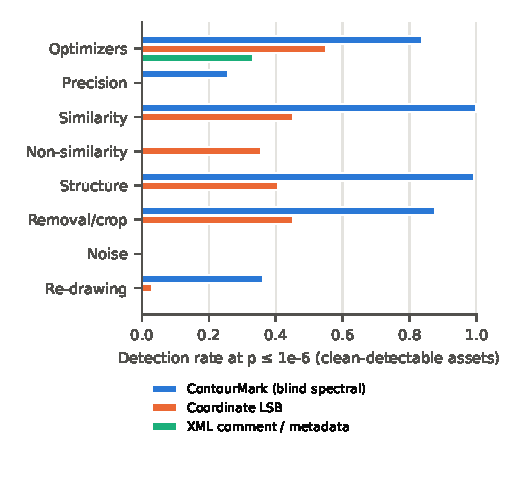
\includegraphics[width=\columnwidth]{figures/attack_groups.pdf}
\caption{Detection at $p\le10^{-6}$ by attack family, conditional on clean detection for each method (900 test assets).}
\label{fig:attacks}
\end{figure}

\subsection{Calibration}
For each unmarked test document we computed the geometric observations once and scored them under 300 independent keys, giving 268{,}200 null tests over 894 documents with at least one carrier. Observed rates were:
\begin{itemize}
\item 6.9\% at $\alpha{=}10^{-1}$;
\item 0.68\% at $10^{-2}$;
\item 0.063\% at $10^{-3}$;
\item $4.5\times10^{-5}$ at $10^{-4}$;
\item $1.1\times10^{-5}$ (3 hits) at $10^{-5}$.
\end{itemize}
The bound holds or is met within sampling noise at every level. The smallest null p-value was $9.3\times10^{-7}$. Under exact calibration the expected count at $10^{-6}$ is at most 0.27, so observing one has probability about 0.24. The per-asset nulls in the main run agree (Figure~\ref{fig:null}): the unmarked original with the owner key gives 0.6\% at $10^{-2}$ and none at $10^{-6}$; the marked file with a wrong key gives none at $10^{-6}$.

\begin{figure}[t]
\centering
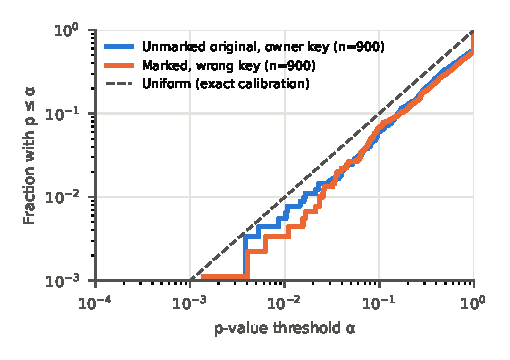
\includegraphics[width=\columnwidth]{figures/null_calibration.pdf}
\caption{Empirical null CDF of reported p-values (log--log). Points on or below the diagonal indicate a valid, conservative bound.}
\label{fig:null}
\end{figure}

\subsection{Fidelity, size, and cost}
\textbf{Distortion.}
\begin{itemize}
\item The median maximum curve displacement is 0.31\% of the drawing diagonal (95th percentile 0.77\%): about 0.3\,px when a full-canvas icon is rendered at 64\,px, 1.1\,px at 256\,px, and 4.5\,px at 1024\,px.
\item Median SSIM is 0.985 at 256\,px and 0.979 at 1024\,px; PSNR is 28.8 and 25.3\,dB.
\item PSNR is dominated by sub-pixel edge shifts on high-contrast line art. Side-by-side renders show no visible change at typical icon sizes.
\item A perceptual study remains necessary before making an imperceptibility claim for large renders.
\end{itemize}

\textbf{Size and time.}
\begin{itemize}
\item Marked files are $1.8\times$ the original after SVGO, a median of 389 added bytes. The cost comes from curve subdivision and higher-precision coordinates.
\item Embedding takes 0.23\,s and detection 0.025\,s (medians, one core).
\end{itemize}

\textbf{Operating curve.} On the development split, the lattice step trades these costs directly:

\medskip
\noindent{\small\begin{tabular}{@{}lrrrrr@{}}
\toprule
$\Delta$ & Max shift & PSNR & SVGO & 2\,dp & 0.1\% noise\\
 & (\% diag) & @1024 & & & \\
\midrule
0.002 & 0.2 & 29.7 & 86\% & 53\% & 0\%\\
0.004 & 0.3 & 25.8 & 92\% & 74\% & 0\%\\
0.016 & 1.2 & 18.0 & 100\% & 90\% & 43\%\\
\bottomrule
\end{tabular}}
\medskip

Larger bands ($k{=}2..13$) and lower gain thresholds changed clean coverage by at most 1.1 points while increasing size, so the defaults use the smaller band.

\subsection{LLM-written SVG}
On 40 SVGs written by Qwen~3.5 4B, \system{} detects 100\% clean, 100\% after SVGO, and 93\% after 2-decimal rounding (median $p=10^{-21}$, six marked contours), with PSNR 38\,dB at 1024\,px. Byte overhead after SVGO is larger ($2.9\times$) because these files use basic shapes, which are rewritten as paths. Rasterize-and-retrace removes the mark from these overlapping colour drawings.

\subsection{Informed attacker (A2)}
An attacker who knows the algorithm and $\Delta$ but not $K$ re-embeds with a random key. On 228 detectable assets (30 per source) this removes the mark in every case. The attack's distortion (median PSNR 26.5\,dB at 1024\,px) equals that of embedding (25.4\,dB). Plain QIM with public $\Delta$ offers no margin against this attacker. Spread-transform dither modulation over keyed projections of the band is the standard remedy: it raises an uninformed re-quantizer's required distortion by roughly $\sqrt{L}$ for $L$ spread coefficients. We leave it to future work and scope our claims to A0 and A1 transformations.

\section{Limitations}
\begin{itemize}
\item \textbf{Capacity.} Straight-line icons (a Lucide ``minus'') carry nothing under a similarity-invariant carrier that keeps lines straight. Coverage is 69--92\% by source. Relationships between contours (relative placement of strokes) are an unexploited carrier.
\item \textbf{Similarity invariance only.} Non-uniform scaling and skew remove the mark. Per-contour affine normalization is possible but is unstable for thin contours.
\item \textbf{Stroke outlining and retracing.} Converting strokes to filled outlines (picosvg, Illustrator ``Outline Stroke'') keeps 78\% of marks. Rasterize-and-retrace keeps at most 24\%. A raster-domain decoder, as in FontCode and DeepMorph, would complement the geometric detector.
\item \textbf{Informed removal.} Re-quantization with a random key removes the mark at embedding-level distortion (\S5.6).
\item \textbf{Seed classes.} Common shapes such as circles share seed classes across assets. An attacker holding many marked circles could estimate their lattice. Per-provider key rotation limits this; we have not measured it.
\item \textbf{Evidence, not authorship.} A positive test shows that geometry marked with $K$ is present, including after copy-and-paste into other work. Keys should be committed with timestamps if results are used as evidence.
\item \textbf{Fidelity.} Distortion is measured with pixel metrics, and a perceptual study is still needed. Byte overhead ($1.8\times$ after SVGO) matters for icon sprites.
\end{itemize}

\section{Related work}
\textbf{Vector graphics.} Solachidis and Pitas, and Doncel, Nikolaidis and Pitas (TVCG 2007) watermark Fourier-descriptor magnitudes of \emph{vertex sequences} with correlation detection. They are the closest prior art to our invariants. Their carrier depends on the representation, and host interference requires hundreds of vertices; our re-implementation fails at icon scale. A 2024 V-system method represents Bézier curves exactly and reports transformation robustness only. GIS vector-map schemes quantize per-vertex angles or distance ratios with QIM and target simplification and cropping on dense maps. Blinova and Urbanovich hide data in cubic split ratios; this is lossless in rendering but fragile to re-parameterization and rounding.

\textbf{Raster-decoded vector marks.} FontCode, AutoStegaFont, GlyphShield, and DeepMorph learn perturbations of glyphs or drawings decoded from images, and target screenshots and print-scan. They need trained decoders and use empirical thresholds. They are complementary to our geometry-domain detector for the rasterize-and-retrace threat.

\textbf{Quantization watermarking.} Chen and Wornell's QIM and dither modulation remove host interference. Spread-transform DM raises the cost of uninformed re-quantization. Content-derived keys (Fridrich) prevent pooling.

\textbf{Generative-model marks.} SynthID-Text, green-list, and Gumbel samplers mark tokens at inference; code watermarks fail under semantics-preserving rewrites. Image watermarks (Stable Signature, Tree-Ring, TrustMark, VINE) face regeneration attacks. Impossibility results bound what any scheme can claim.

\section{Conclusion}
Moving the mark from SVG syntax to drawn geometry turns the optimizer, the chief obstacle to SVG provenance, into a near no-op. A radial-function spectral carrier, keyed QIM, a representation-free capacity model, and an exactly calibrated detector give a post-hoc watermark that applies to any SVG generator. It is detectable from the file and key alone and survives the benign pipeline where every syntax-level baseline fails. The measured limits (capacity on straight-line icons, noise at the mark's own amplitude, non-similarity warps, retracing, informed re-quantization) define the next steps: inter-contour carriers, spread-transform hardening, and a raster-domain decoder.

\end{document}
